\documentclass{article}


\setlength{\textwidth}{16cm}
\setlength{\topmargin}{-1cm}
\setlength{\evensidemargin}{0cm}
\setlength{\oddsidemargin}{0cm}
\setlength{\textheight}{22.5cm}
\usepackage[utf8]{inputenc}
\usepackage[T1]{fontenc}
\usepackage{charter} % very clean and readable font
\usepackage{courier}
\usepackage{unicode-chars}



\usepackage[show]{ed}  % set to hide for producing a released version

\usepackage{alltt}
\usepackage{casl}
\usepackage{xspace}
\usepackage{color}
\usepackage{url}
\usepackage{threeparttable,hhline}
\usepackage{tabularx}
\usepackage{paralist}
\usepackage{listings}
\lstset{basicstyle=\ttfamily,columns=fixed}

\usepackage[pdfborder=0 0 0,bookmarks,
pdfauthor={Till Mossakowski, Christian Maeder, Mihai Codescu, Eugen Kuksa, Christoph Lange},
pdftitle={Hets for Common Logic Users}]
{hyperref} %% do not load more packages after this line!!

\input{xy}
\xyoption{v2}

\newcommand{\QUERY}[1]%{}
{\marginpar{\raggedright\hspace{0pt}\small #1\\~}}

\newcommand{\eat}[1]{}

\newenvironment{EXAMPLE}[1][]   {\par#1\begin{EXAMPLEFORMAT}\begin{ITEMS}}
                                {\end{ITEMS}\end{EXAMPLEFORMAT}\par}
\newcommand{\IEXT}[1]           {\\#1\I}
\newcommand{\IEND}              {\I\END}
\newenvironment{EXAMPLEFORMAT}  {}{}

%% Added by MB to have some extra vertical space after the ``main'' examples
%% following the points (and some others in the text):
\newenvironment{BIGEXAMPLE}   {\begin{EXAMPLE}} {\end{EXAMPLE}\medskip}
\newenvironment{DETAILS}[1][]   {#1\begin{DETAILSFORMAT}}{\end{DETAILSFORMAT}}
\newenvironment{DETAILSFORMAT}  {}{}
\newenvironment{META}[1][]      {#1\begin{METAFORMAT}}{\end{METAFORMAT}}
\newenvironment{METAFORMAT}     {\medskip\vrule\hspace{1ex}\vrule\hspace{1ex}%
                                 \begin{minipage}{0.9\textwidth}\it}
                                {\end{minipage}\par\medskip}

\newcommand{\SLIDESMALL}        {}
\newcommand{\SLIDESONLY}[1]     {}


%%%%%%%%%%%%%%%%%%%%%%%%%%%%%%%%%%%%%%%%%%%%%%%%%%%%%%%%%%%%%%%%%%%%%%
% SIMULATING SMALL-CAPS FOR BOLD, EMPH

\newcommand{\normalTEXTSC}[2]{{#1\scriptsize#2}}
%% NOT \newcommand{\normalTEXTSC}[2]{{\normalsize#1\scriptsize#2}}
\newcommand{\largeTEXTSC} [2]{{\large     #1\small     #2}}
\newcommand{\LargeTEXTSC} [2]{{\Large     #1\normalsize#2}}
\newcommand{\LARGETEXTSC} [2]{{\LARGE     #1\large     #2}}
\newcommand{\hugeTEXTSC}  [2]{{\huge      #1\Large     #2}}
\newcommand{\HugeTEXTSC}  [2]{{\Huge      #1\LARGE     #2}}


%\newcommand     {\CASL}{\normalTEXTSC{C}{ASL}\xspace}
\newcommand{\largeCASL} {\largeTEXTSC{C}{ASL}\xspace}
\newcommand{\LargeCASL} {\LargeTEXTSC{C}{ASL}\xspace}
\newcommand{\LARGECASL} {\LARGETEXTSC{C}{ASL}\xspace}
\newcommand {\hugeCASL}  {\hugeTEXTSC{C}{ASL}\xspace}
\newcommand {\HugeCASL}  {\HugeTEXTSC{C}{ASL}\xspace}

%\newcommand     {\CoFI}{CoFI\xspace}

\newcommand     {\MAYA}{\normalTEXTSC{M}{AYA}\xspace}
\newcommand{\largeMAYA} {\largeTEXTSC{M}{AYA}\xspace}

\newcommand     {\Hets}{\normalTEXTSC{H}{ETS}\xspace}
\newcommand{\largeHets} {\largeTEXTSC{H}{ETS}\xspace}
\newcommand{\LARGEHets} {\LARGETEXTSC{H}{ETS}\xspace}

\newcommand     {\Cats}{\normalTEXTSC{C}{ATS}\xspace}
\newcommand{\largeCats} {\largeTEXTSC{C}{ATS}\xspace}

\newcommand     {\ELAN}{\normalTEXTSC{E}{LAN}\xspace}
\newcommand{\largeELAN} {\largeTEXTSC{E}{LAN}\xspace}

\newcommand     {\HOL}{\normalTEXTSC{H}{OL}\xspace}
\newcommand{\largeHOL} {\largeTEXTSC{H}{OL}\xspace}

\newcommand     {\Isabelle}{\normalTEXTSC{I}{SABELLE}\xspace}
\newcommand{\largeIsabelle} {\largeTEXTSC{I}{SABELLE}\xspace}

\newcommand     {\SPASS}{\normalTEXTSC{S}{PASS}\xspace}

\newcommand     {\Horn}{\normalTEXTSC{H}{ORN}}

%%%%% Klaus macros
\newcommand{\CASLDL}{\textmd{\textsc{Casl-DL}}\xspace}
\newcommand{\Dolce}{\textmd{\textsc{Dolce}}\xspace}
\newcommand{\SHOIN}{$\mathcal{SHOIN}$(\textbf{D})\xspace}
\newcommand{\SROIQ}{$\mathcal{SROIQ}$(\textbf{D})\xspace}
\newcommand{\DL}{DL\xspace}
%%%%% end of Klaus macros

%% Use \ELAN-\CASL, \HOL-\CASL, \Isabelle/\HOL

\newcommand{\LCF}{LCF\xspace}

\newcommand{\ASF}{ASF\xspace}
%%\newcommand     {\ASF}{\normalTEXTSC{A}{SF}\xspace}
%%\newcommand{\largeASF} {\largeTEXTSC{A}{SF}\xspace}

\newcommand{\SDF}{SDF\xspace}
%%\newcommand     {\SDF}{\normalTEXTSC{S}{DF}\xspace}
%%\newcommand{\largeSDF} {\largeTEXTSC{S}{DF}\xspace}

\newcommand     {\ASFSDF}{\normalTEXTSC{A}{SF}+\normalTEXTSC{S}{DF}\xspace}
\newcommand{\largeASFSDF} {\largeTEXTSC{A}{SF}+\largeTEXTSC{S}{DF}\xspace}

\newcommand     {\HasCASL}{\normalTEXTSC{H}{AS}\normalTEXTSC{C}{ASL}\xspace}
\newcommand{\largeHasCASL} {\largeTEXTSC{H}{AS}\largeTEXTSC{C}{ASL}\xspace}

%% Do NOT use \ASF+\SDF (it gives a superfluous space in the middle)

\newcommand{\CCC}{CCC\xspace}

\newcommand{\CoCASL}{\normalTEXTSC{C}{O}\normalTEXTSC{C}{ASL}\xspace}
\newcommand{\CspCASL}{\normalTEXTSC{C}{SP}-\normalTEXTSC{C}{ASL}\xspace}
\newcommand{\Csp}{\normalTEXTSC{C}{SP}\xspace}
\newcommand{\CcsCASL}{CCS-\normalTEXTSC{C}{ASL}\xspace}
\newcommand{\CASLLtl}{\normalTEXTSC{C}{ASL}-\normalTEXTSC{L}{TL}\xspace}
\newcommand{\CASLChart}{\normalTEXTSC{C}{ASL}-\normalTEXTSC{C}{HART}\xspace}
\newcommand{\SBCASL}{\normalTEXTSC{S}{B}-\normalTEXTSC{C}{ASL}\xspace}
\newcommand{\HetCASL}{\normalTEXTSC{H}{ET}\normalTEXTSC{C}{ASL}\xspace}
\newcommand{\ModalCASL}{\normalTEXTSC{M}{odal}\normalTEXTSC{C}{ASL}\xspace}


\begin{document}

\title{{\bf \protect{\LARGEHets} for Common Logic Users}\\
-- Version 0.99 --}
\author{Till Mossakowski, Christian Maeder,
  Mihai Codescu, Eugen Kuksa, Christoph Lange\\[1em]
DFKI GmbH, Bremen, Germany.\\[1em]
Comments to: \href{mailto:hets-users@informatik.uni-bremen.de}{hets-users@informatik.uni-bremen.de} \\
(the latter needs subscription to the mailing list)
}

\maketitle

\setcounter{tocdepth}{1}
\tableofcontents

\section{Introduction}

Common Logic (CL) is an ISO standard published as ``ISO/IEC 24707:2007
--- Information technology — Common Logic (CL): a framework for a family
of logic-based languages'' \cite{CommonLogic:oldfashioned}. CL is based on untyped first-order
logic, but extends first-order logic in two ways: \begin{inparaenum}[(1)]\item any term can be
used as function or predicate, and \item sequence markers allow
for talking about sequences of individuals directly\end{inparaenum}.\footnote
{Strictly speaking, only the second feature goes beyond first-order
logic.}

The Heterogeneous Tool Set (\Hets) is an open source software providing
several kinds of tool support for Common Logic:
\begin{itemize}
\item a parser for the Common Logic Interchange Format (CLIF) --- CLIF
  is a Lisp-like syntax for CL;
\item a connection of CL to well-known first-order theorem provers
like SPASS, darwin and Vampire, such that logical consequences
of CL theories can be proved;
\item a connection of CL to the higher-order provers Isabelle/HOL
and Leo-II in order to perform induction proofs in theories
involving sequence markers;
\item a connection to first-order model finders like darwin that
allow one to find models for CL theories;
\item support for proving interpretations between CL theories to be correct;
\item a translation that eliminates the use of CL modules\footnote{Actually, we are using a revised semantics for modules, as proposed
recently in~\cite{NH:CommonLogicHoratio}.}. Since the semantics of CL modules
is special to CL, this elimination of modules is necessary before
sending CL theories to a standard first-order prover;
\item a translation of the Web Ontology Language OWL to CL;
\item a translation of propositional logic to CL.
\end{itemize}

This guide will introduce you to these functionalities of \Hets.
For the full functionalities of \Hets, see the \Hets user guide  
\cite{HetsUserGuide}.


\section{The Heterogeneous Tool Set and Its Input Languages}

The central idea of the Heterogeneous Tool Set (\protect\Hets) is to
provide a general framework for formal methods integration and proof
management. One can think of \Hets acting like a motherboard where
different expansion cards can be plugged in, the expansion cards here
being individual logics (with their analysis and proof tools) as well
as logic translations. The \Hets motherboard already has plugged in
a number of expansion cards (e.g., the theorem provers Isabelle, SPASS
and more, as well as model finders). Hence, a variety of tools is
available, without the need to hard-wire each tool to the logic at
hand.
\begin{figure}
\begin{center}
  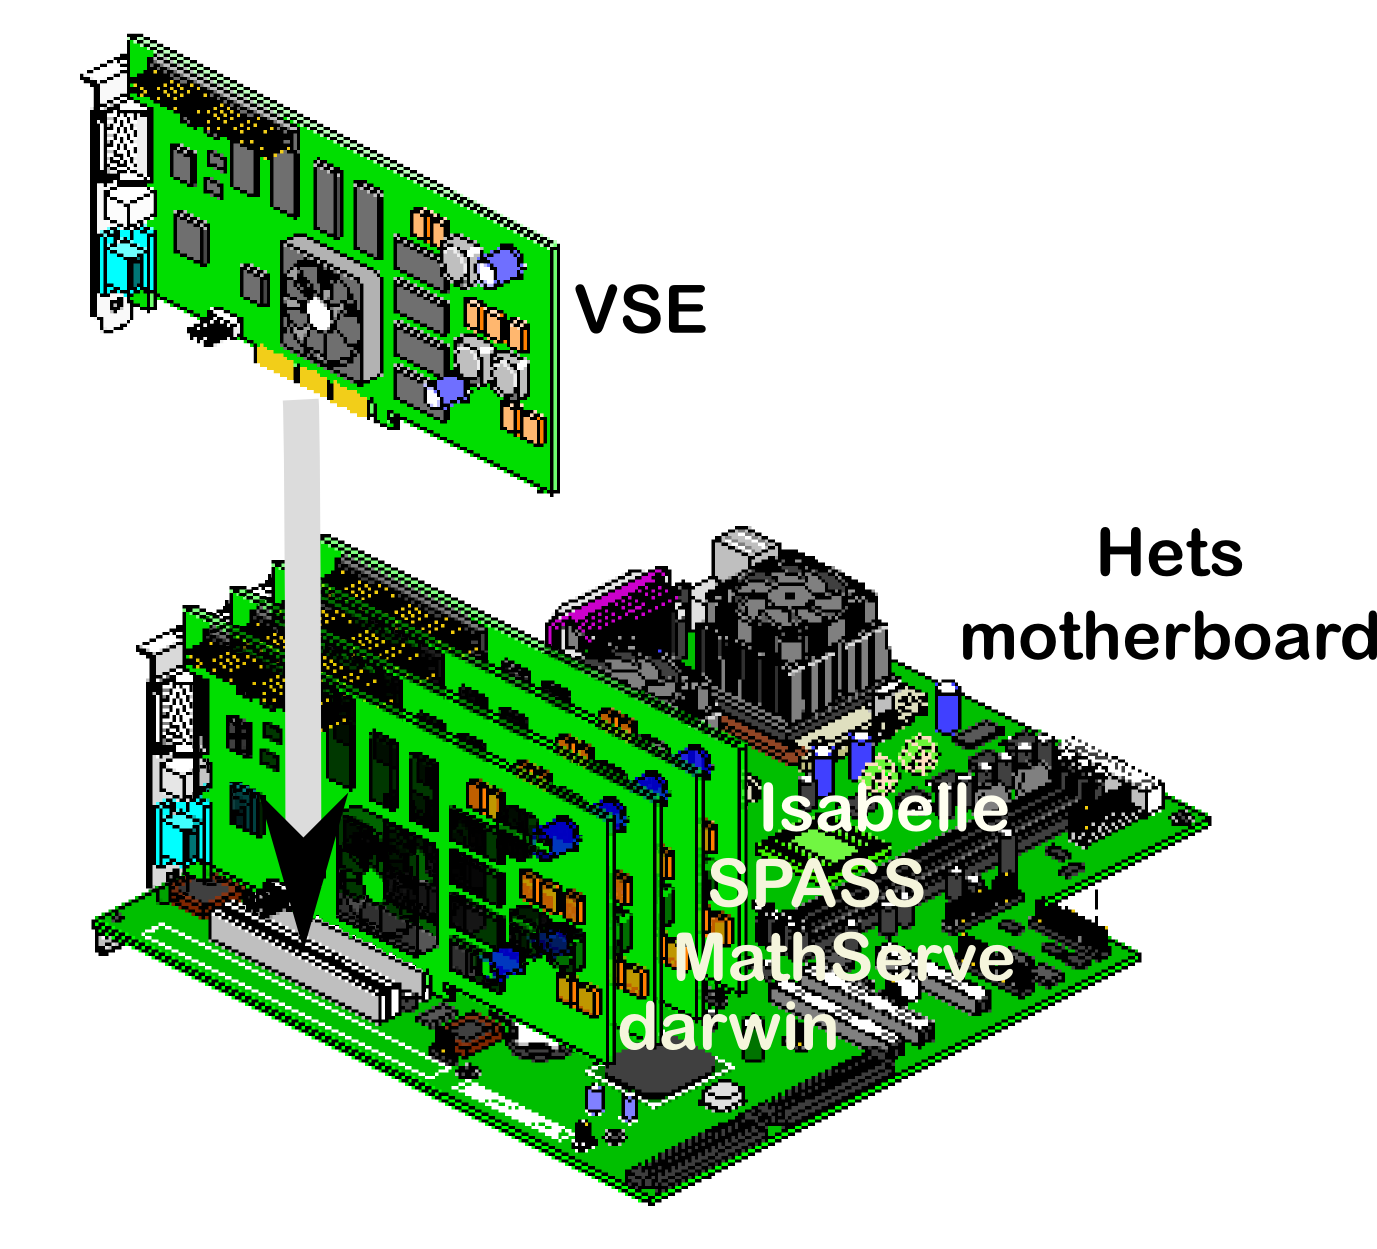
\includegraphics[width=0.45\textwidth]{hets-motherboard}
\end{center}
\caption{The \Hets motherboard and some expansion cards}
\end{figure}

\Hets consists of logic-specific tools for the parsing and static
analysis of the different involved logics, as well as a
logic-independent parsing and static analysis tool for structured and
architectural specifications and libraries. The latter of course needs
to call the logic-specific tools whenever a basic specification is
encountered.

\Hets is based on the theory of institutions \cite{GoguenBurstall92},
which formalise the notion of a logic. The theory behind \Hets is laid
out in \cite{Habil}. A short overview of \Hets is given in
\cite{MossakowskiEA06,MossakowskiEtAl07b}.

\Hets supports a number of input languages directly, such as Common
Logic and OWL2 and \HetCASL. They will be described in the next
sections.

\subsection{Common Logic and the Common Logic Interchange Format (CLIF)}

CLIF is specified in Annex A of the Common Logic standard
\cite{CommonLogic:oldfashioned}. \Hets can directly read in files in
CLIF syntax, and also recursively reads in any imported files (cf.\ Sect.~\ref{relationsInCL} for the syntax).

Common Logic itself does not support the specification of logical
consequences, nor relative theory interpretations, nor other
features that speak about structuring and comparing logical
theories. Michael Gr\"uninger has suggested certain special annotations comments for
this purpose, which are supported by \Hets, see
Sect.~\ref{relationsInCL}.  Alternatively, CLIF syntax can be used
for specifications within \HetCASL files, or CLIF files can be referred to within \HetCASL
files.  \HetCASL is a structuring language supporting relative theory
interpretations and other things, see Sect.~\ref{HetCASL} below.

\subsection{OWL2}

OWL2 is a W3C standard \cite{w3c:owl2-overview}.
\Hets can directly read in OWL2 files in all syntaxes (called ``serialisations'') that the OWL API supports \cite{OWLAPI:URL}, including
the native OWL XML syntax \cite{w3c:owl2-xml},  the human-readable
Manchester syntax \cite{w3c:owl2-manchester}, as well as RDF \cite{w3c:owl2-RDF-mapping}.  The RDF data model has multiple possible syntaxes itself, including RDF/XML \cite{w3c04:rdf-xml} and the text-oriented Turtle syntax \cite{w3c:turtle}.

Since OWL2 does not support relative theory interpretations and other
structuring features, such things can only be expressed in \HetCASL
files. For this purpose, OWL2 Manchester syntax can be used within
\HetCASL files, or OWL2 files can be referred to within \HetCASL files.

\subsection{HetCASL}
\label{HetCASL}
For heterogeneous specification, \Hets offers the Heterogeneous
language \HetCASL.  \HetCASL is not so much a logic, but a meta
language that can express relations of theories written in different
logics, like logical consequences, relative interpretations of
theories, conservative extensions, translations of theories
along logic translations, etc.

 \HetCASL generalises the structuring
constructs of
\CASL (Common Algebraic Specification Language \cite{CASL-UM,CASL/RefManual}) to arbitrary logics
(if they are formalised as institutions and plugged into
the \Hets motherboard), as well as to heterogeneous
combinations of specifications written in different logics.
See
Fig.~\ref{fig:lang} for a simple subset of the
\HetCASL syntax, where \emph{basic specifications} are unstructured
specifications or modules written in a specific logic.  The graph of
currently supported logics and logic translations (the latter are also
called comorphisms) is shown in Fig.~\ref{fig:LogicGraph}, and the
degree of support by \Hets in Fig.~\ref{fig:Languages}.

% We give an ad hoc listing language definition of EBNF here.  This should probably go into lstlang0.sty.
\begin{lstlisting}[float,label={fig:lang},caption={Syntax of a simple subset of the heterogeneous specification language. \texttt{BASIC-SPEC} and \texttt{SYMBOL-MAP} have a logic specific syntax, while \texttt{ID} stands for some form of identifiers.},basicstyle=\ttfamily\small,morecomment={[l]{\%\%\ }},morekeywords={then,with,logic,spec,end,view,to},escapeinside={<>}]
SPEC ::= BASIC-SPEC        %% logic-specific syntax, e.g. CLIF or Manchester syntax
       | SPEC then SPEC          %% extension of a spec with new symbols and axioms
       | SPEC then %implies SPEC %% annotation: extension is logically implied
       | SPEC with SYMBOL-MAP    %% renaming of SPEC along SYMBOL-MAP
       | SPEC with logic ID      %% translation of SPEC to a different logic

DEFINITION ::= logic ID            %% select a new logic for subsequent items
             | spec ID = SPEC end  %% give the name ID to SPEC
             | view ID : SPEC to SPEC = SYMBOL-MAP end
               %% interpretation of theories
             | view ID : SPEC to SPEC = logic ID end
               %% dto., but across different logics

LIBRARY = DEFINITION*
\end{lstlisting}

With \emph{heterogeneous structured specifications}, it is possible to
combine and rename specifications, hide parts thereof, and also
translate them to other logics. \emph{Architectural specifications}
prescribe the structure of implementations.  \emph{Specification
  libraries} are collections of named structured and architectural
specifications. \emph{Refinements} express the fact the a specification
is becoming more specific. All this is supported by \HetCASL.
For details, see \cite{Mossakowski04,Habil,CASL/RefManual}.


\section{Logics supported by Hets}

\Hets supports a variety of different logics.   The following are most important for use with Common Logic:


\begin{figure}
  \begin{center}
    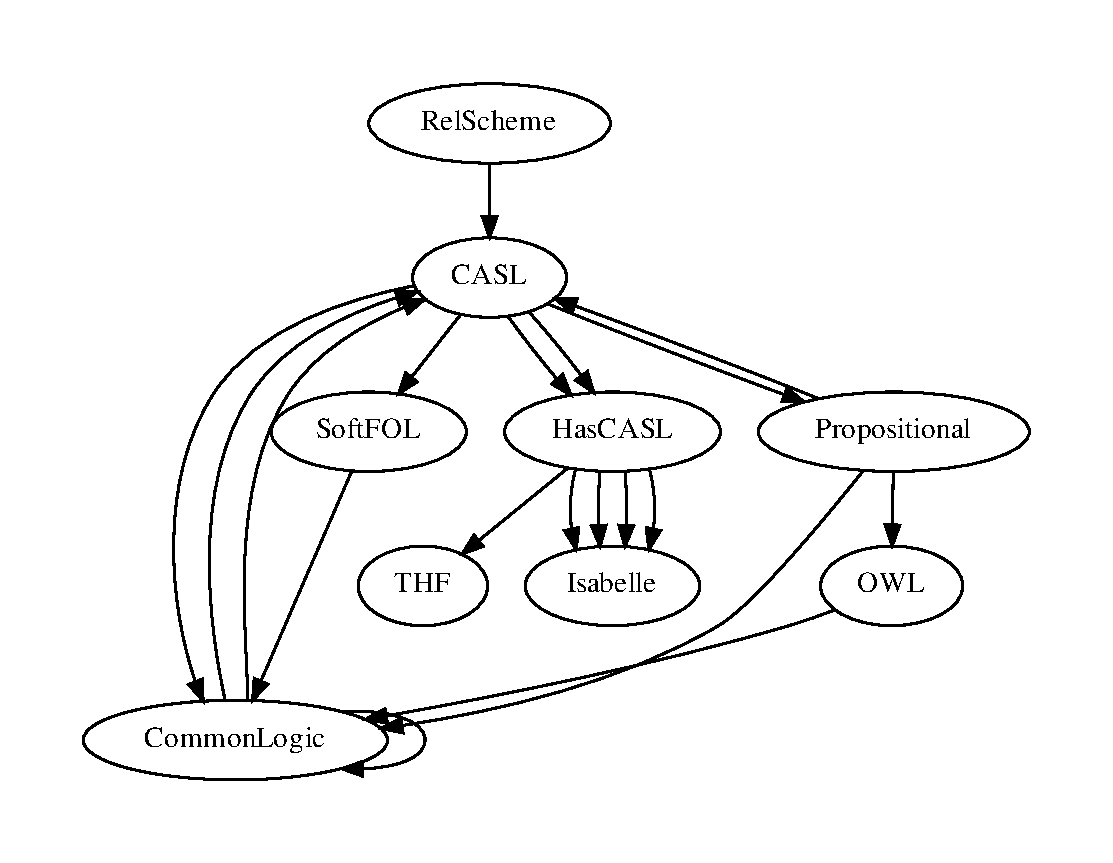
\includegraphics[width=.67\textwidth]{LogicGraph-CL}
  \end{center}
\caption{Graph of logics related to Common Logic that are currently supported by \Hets. The more an
ellipse is filled with green, the more stable is the implementation of the
logic. Blue indicates a prover-supported logic.}
\label{fig:LogicGraph}
\end{figure}

\begin{figure}
\begin{center}
\begin{tabular}{|l|c|c|c|}\hline
Language & Parser & Static Analysis & Prover \\\hline
\CASL & x & x & -- \\\hline
Common Logic & x (CLIF) & x & -- \\\hline
OWL2 & x & x & x \\\hline
Propositional & x & x & x \\\hline
SoftFOL & x & -- & x \\\hline
\end{tabular}
\end{center}
\caption{Current degree of \Hets support for some of the languages.
Languages without prover can still ``borrow'' provers
via logic translations.\label{fig:Languages}}
\end{figure}

\begin{description}


\item[Common Logic] is an ISO standard published as ``ISO/IEC 24707:2007 - Information technology — Common Logic (CL): a framework for a family of logic-based languages'' \cite{CommonLogic:oldfashioned}. It is based on first-order logic, but extends first-order
logic in several ways.   The Common Logic
  Interchange Format (CLIF) provides a Lisp-like syntax for Common
  Logic.  \Hets currently only supports parsing CLIF. If you need
  other dialects, send us a message and we will add them.

\item[OWL2] is the Web Ontology Language recommended by the
  World Wide Web Consortium (W3C, \url{http://www.w3c.org}); see \cite{w3c:owl2-overview}. It is
  used for knowledge representation on the Semantic Web
  \cite{berners:2001:SWeb}.
Hets calls an external OWL2 parser
  written in Java to obtain the abstract syntax for an OWL file and its
  imports. The Java parser also does a first analysis classifying
  the OWL ontology into the sublanguages OWL Full (all of OWL, under the RDF semantics, undecidable \cite{w3c:owl2-rdf-based-semantics}), OWL DL (all of OWL, under the direct semantics \cite{w3c:owl2-direct-semantics}), and the so-called OWL Profiles (i.e.\ proper sublanguages) OWL EL, OWL QL, and OWL RL \cite{w3c:owl2-profiles}.
 Hets supports all except OWL Full.
The
  structuring of the OWL imports is displayed as a Development Graph.

\item[Propositional] is classical propositional logic, with
the zChaff SAT solver \cite{Herbstritt03} connected to it.

\item[SoftFOL] \cite{LuettichEA06a} offers several automated theorem
  proving (ATP) systems for first-order logic with equality: \begin{inparaenum}[(1)]\item \SPASS
  \cite{WeidenbachEtAl02}, see \url{http://www.spass-prover.org}; 
\item Vampire \cite{RiazanovV02} see \url{http://www.vprover.org};
\item Eprover \cite{Schulz:AICOM-2002}, see \url{http://www.eprover.org};
\item E-KRHyper \cite{DBLP:conf/cade/PelzerW07}, see \url{http://www.uni-koblenz.de/~bpelzer/ekrhyper}, and 
\item 
  MathServe Broker\footnote{which chooses an appropriate ATP upon a
    classification of the FOL problem} \cite{ZimmerAutexier06}.
\end{inparaenum}
  These together comprise some of the most advanced theorem provers
  for first-order logic. SoftFOL is essentially the first-order
  interchange language TPTP \cite{DBLP:conf/lpar/Sutcliffe10},
see \url{http://www.tptp.org}.

\item[CASL] extends many sorted first-order logic with partial
  functions and subsorting.  It also provides induction sentences,
  expressing the (free) generation of datatypes.
For more details on \CASL see \cite{CASL/RefManual,CASL-UM}.
For Common Logic, \CASL can be seen as kind of transitional hub, linking
Common Logic to other logics, most importantly SoftFOL.

\item[\Isabelle] \cite{NipPauWen02} is the logic of the interactive
  theorem prover Isabelle for higher-order logic.

\item[THF] is an interchange language for higher-order logic
  \cite{DBLP:conf/cade/BenzmullerRS08}, similar to what TPTP
  is for first-order logic. \Hets connects THF to the automated
  higher-order prover Leo-II.

\item[HasCASL] is a higher order extension of \CASL allowing
  polymorphic datatypes and functions. It is closely related to the
  programming language Haskell and allows program constructs being
  embedded in the specification. For Common Logic, \HasCASL
  is mainly interesting as a transitional hub for paths
  to the provers Isabelle and Leo-II.

\item[RelScheme] is a logic for relational databases \cite{DBLP:journals/ao/SchorlemmerK08}.

\end{description}

Various logics are supported with proof tools. Proof support for the
other logics can be obtained by using logic translations to a
prover-supported logic. For Common Logic, the paths to SoftFOL
are particularly interesting, because this offers an interface
to standard first-order provers. Moreover, the paths to THF
and Isabelle offer interfaces to higher-order provers, which
is essential if you want to prove inductive theorems about
sequences.


An introduction to \CASL can be found in the \CASL User Manual
\cite{CASL-UM}; the detailed language reference is given in
the \CASL Reference Manual \cite{CASL/RefManual}.  These documents
explain both the \CASL logic and language of basic specifications as
well as the logic-independent constructs for structured and
architectural specifications.  The corresponding document explaining the
\HetCASL language constructs for \emph{heterogeneous} structured specifications
is the \HetCASL language summary \cite{Mossakowski04}; a formal
semantics as well as a user manual with more examples are in preparation.
Some of \HetCASL's heterogeneous constructs will be illustrated
in Sect.~\ref{sec:HetSpec} below.\\

For further information on logics supported by \Hets, see the \Hets user guide  
\cite{HetsUserGuide}.

\section{Logic translations supported by Hets}
\label{comorphisms}

Logic translations (formalised as institution comorphisms
\cite{GoguenRosu02}) translate from a given source logic to a given
target logic. More precisely, one and the same logic translation
may have several source and target \emph{sub}logics: for
each source sublogic, the corresponding sublogic of the target
logic is indicated.

In more detail, the following list of logic translations involving Common Logic 
is currently supported by \Hets:\\

\noindent\begin{tabularx}{\textwidth}{|l|X|}\hline
CommonLogic2CASL & Coding Common Logic to \CASL. Module elimination
		   is applied before translating to \CASL. \\\hline
CommonLogic2CASLCompact & Coding compact Common Logic to \CASL. 
			  Compact Common Logic is a sublogic of Common Logic
			  where no sequence markers occur. Module elimination
			  is applied before translating to \CASL. We recommend
			  using this comorphism whenever possible because it 
			  results in simpler specifications.\\\hline
CommonLogicModuleElimination & Eliminating modules from a Common Logic theory 
			       resulting in an equivalent specification without
				modules. \\\hline
OWL22CommonLogic & Inclusion of OWL2 description logic \\\hline
Prop2CommonLogic & Inclusion of propositional logic \\\hline
SoftFOL2CommonLogic & Inclusion of first order logic \\\hline
CASL2SoftFOL & Coding of CASL.SuleCFOL=E to SoftFOL \cite{LuettichEA06a},
mapping types to soft types \\\hline
CASL2SoftFOLInduction & Same as CASL2SoftFOL but with instances of induction
axioms for all proof goals \\\hline
CASL2SoftFOLInduction2 & Similar to CASL2SoftFOLInduction but replaces goals with induction premises \\\hline
CASL2Propositional & Translation of propositional FOL \\\hline
\end{tabularx}\\

Those comorphisms can be chained, e.g., for theorem proving, you can translate 
Common Logic to SoftFOL with \texttt{CommonLogic2CASLCompact;CASL2SoftFOLInduction} 
since there is no prover for Common Logic or \CASL.

For further information on logic translations supported by \Hets, see the \Hets 
user guide \cite{HetsUserGuide}.

\section{Getting started}

The latest \Hets version can be obtained from the
\Hets tools home page
\begin{quote}
\url{http://www.dfki.de/sks/hets}
\end{quote}
 Since \Hets is being
improved constantly, it is recommended always to use the latest version.

\Hets is currently available (on Intel architectures only) for Linux
and Mac OS X.

There are several possibilities to install \Hets.
\begin{enumerate}
\item
The best support is currently given via Ubuntu packages.
For Ubuntu Lucid Lynx, enter the following into a terminal:
\begin{lstlisting}
sudo apt-add-repository ppa:hets/hets
sudo apt-add-repository \
  "deb http://archive.canonical.com/ubuntu lucid partner"
sudo apt-get update
sudo apt-get install hets
\end{lstlisting}
For later Ubuntu versions, replace lucid by maverick, natty or oneiric.

This will also install quite a couple of tools for proving requiring about
800 MB of disk space. For a minimal installation use \texttt{apt-get install
  hets-core} instead of \texttt{hets}.
\item For Mac OS X 10.6 (Snow Leopard) we provide a meta package
  \texttt{Hets.mpkg} based on MacPorts that will be extended by further tools
  for proving in the future.
\item
Then we have Java based \Hets installer that we may drop in the future.
Download a \texttt{.jar} file and start it with
\begin{lstlisting}
java -jar file.jar
\end{lstlisting}
Note that you need Sun/Oracle Java 1.4.2 or later. On a Mac, you can just
double-click on the \texttt{.jar} file, but you have to install the MacPorts
\texttt{libglade2} package (and all its dependencies) yourself. In order to
speed this up we provide a meta package \texttt{libglade2.mpkg}, too.

The installer will lead you through the installation with
a graphical interface. It will download and install further
software (if not already installed on your computer):

\medskip
{\small
\begin{tabularx}{\linewidth}{|l|l|X|}\hline
Hets-lib & specification library & \url{http://www.cofi.info/Libraries}\\\hline
uDraw(Graph) & graph drawing & \url{http://www.informatik.uni-bremen.de/uDrawGraph/en/}\\\hline
Tcl/Tk & graphics widget system & (version 8.4 or 8.5 must be installed before)\\\hline
\SPASS & theorem prover & \url{http://spass.mpi-sb.mpg.de/}\\\hline
Darwin & theorem prover & should be installed manually from \url{http://combination.cs.uiowa.edu/Darwin/}\\\hline
\Isabelle & theorem prover & \url{http://www.cl.cam.ac.uk/Research/HVG/Isabelle/}\\\hline
(X)Emacs & editor (for Isabelle) & (must be installed manually)\\\hline
\end{tabularx}
}
\medskip

\item
If you do not have Sun/Oracle Java, you can just download the hets binary.
You have to unpack it with \texttt{bunzip2} and then put it into
some place covered by your \texttt{PATH} environment variable. You also have to
install the above mentioned software and set
several environment variables, as explained on the installation page.

\item
You may compile \Hets from the sources (they are licensed under GPL), 
please follow the
link ``Hets: source code and information for developers''
on the \Hets web page, download the sources (as tarball or from
svn), and follow the
instructions in the \texttt{INSTALL} file, but be prepared to take some time.
\end{enumerate}

Depending on your application further tools are supported and may be
installed in addition:

\medskip
{\small
\begin{tabularx}{\linewidth}{|l|l|X|}\hline
zChaff & SAT solver & \url{http://www.princeton.edu/~chaff/zchaff.html} \\\hline
minisat & SAT solver & \url{http://minisat.se/} \\\hline
Pellet & OWL reasoner & \url{http://clarkparsia.com/pellet/} \\\hline
E-KRHyper & theorem prover
  & \url{http://userpages.uni-koblenz.de/~bpelzer/ekrhyper/} \\\hline
Reduce & computer algebra system
  & \url{http://www.reduce-algebra.com/} \\\hline
Maude & rewrite system & \url{http://maude.cs.uiuc.edu/} \\\hline
VSE & theorem prover & (non-public) \\\hline
Twelf & & \url{http://twelf.plparty.org/} \\\hline
\end{tabularx}
}

\section{Analysis of Specifications}
Consider the following Common Logic text written in CLIF:

\medskip
\begin{lstlisting}[language=clif]
(P x)
(and (P x) (Q y))
(or (Cat x) (Mat y))
(not (On x y))
(if (P x) (Q x))
(exists (z) (and (Pet x) (Happy z) (Attr x z)))
\end{lstlisting}

\Hets can be used for parsing and
checking static well-formedness of specifications.

                \index{parsing}%
                \index{static!analysis}%
                \index{analysis, static}%

Let us assume that the example is in a file named
\texttt{Cat.clif}.
Then you can check the well-formedness of the
specification by typing (into some shell):

\begin{quote}
\texttt{hets Cat.clif}
\end{quote}
\Hets checks both the correctness of this specification
 with respect to the CLIF syntax, as
well as its correctness with respect to the static semantics.
The following flags are available in this context:
\begin{description}
\item[\texttt{-p}, \texttt{-{}-just-parse}] Just do the parsing
 -- the static analysis is skipped and no development graph is created.
\item[\texttt{-s}, \texttt{-{}-just-structured}] Do the parsing and the
  static analysis of (heterogeneous) structured specifications, but
  leave out the analysis of basic specifications.  This can be used
  for prototyping issues, namely to quickly produce a development graph
  showing the dependencies among the specifications (cf.
  Sect.~\ref{sec:DevGraph}) even if the individual specifications are
  not correct yet.
\item[\texttt{-L DIR}, \texttt{-{}-hets-libdir=DIR}]
Use \texttt{DIR} as a colon separated list of directories for specification libraries (equivalently, you can set the variable \texttt{HETS\_LIB} before
calling \Hets).
\end{description}
There are more flags which can be used with \Hets, see \cite{HetsUserGuide}.


\section{Heterogeneous Specification} \label{sec:HetSpec}

\Hets accepts plain text input files (for the 
presented logics) with the following endings:
\\

\begin{tabular}{|l|c|c|}\hline
filename extension & default logic & structuring language\\\hline
\texttt{.casl} & \CASL & \CASL \\\hline
\texttt{.het} & \CASL & \CASL \\\hline
\texttt{.owl} & OWL2 & OWL2 \\\hline
\texttt{.clf} or \texttt{.clif} & CommonLogic & custom, see Sect.~\ref{relationsInCL} \\\hline
\end{tabular}

\medskip

Although the endings \texttt{.casl} and \texttt{.het} are
interchangeable, the former should be used for libraries of
homogeneous \CASL specifications and the latter for \HetCASL libraries
of heterogeneous specifications (that use the \CASL structuring
constructs). Within a \HetCASL library, the current logic can be changed, e.g.,
to Common Logic in the following way:

\begin{lstlisting}[morekeywords=logic]
logic CommonLogic
\end{lstlisting}

The subsequent specifications are then parsed and analysed as
Common Logic specifications. Within such specifications,
it is possible to use references to named \CASL specifications;
these are then automatically translated along the default
embedding of \CASL into Common Logic (cf.\ Fig.~\ref{fig:LogicGraph}).
(There are also heterogeneous constructs
for explicit translations between logics, see \cite{Mossakowski04}.)

The endings \texttt{.clf} and \texttt{.clif} are available for directly reading in
Common Logic CLIF texts, as in the example of \texttt{Cat.clif}.
By contrast, in \HetCASL libraries (ending with \texttt{.het}),
the logic Common Logic has to be chosen explicitly, and the \CASL structuring
syntax needs to be used:

\begin{lstlisting}[language=clif,morekeywords={library,logic,spec,then}]
library Cat

logic CommonLogic

spec Pred = 
. (P x)
  (and (P x) (Q y))

spec Cat =
. (or (Cat x) (Mat y))
  (not (On x y))
  (if (P x) (Q x))

spec PetHappy =
Pred and Cat then
. (exists (z) (and (Pet x) (Happy z) (Attr x z)))
end
\end{lstlisting}

Note that the dot at the beginning of a line indicates that a new text begins.
Hence, it is possible to have multiple texts in a \CASL specification.

This specification is the \HetCASL-structured equivalent to the following three
CLIF files:\footnote{Note that where the Common Logic specification requires ``cl:text'', some samples available on the Web use ``cl-text''. Therefore, \Hets also supports the latter.}\\


\textbf{Pred.clif}:
\begin{lstlisting}[language=clif]
(cl:text Pred 
  (P x)
  (and (P x) (Q y))
)
\end{lstlisting}

\textbf{Cat.clif}:
\begin{lstlisting}[language=clif]
(cl:text Cat 
  (or (Cat x) (Mat y))
  (not (On x y))
  (if (P x) (Q x))
)
\end{lstlisting}

\textbf{Spec.clif}:
\begin{lstlisting}[language=clif]
(cl:text PetHappy 
  (cl:imports Pred) (cl:imports Cat)
  (exists (z) (and (Pet x) (Happy z) (Attr x z)))
)
\end{lstlisting}

Both can be directly used with \Hets, where the former content would be in a 
file with the extension \texttt{.het} and the latter in a file with one of the extensions 
\texttt{.clf} or \texttt{.clif}. This specification is divided into three 
parts, which are linked to each other. These links and some more information can 
be seen in the development graph of the file.


\section{Development Graphs}\label{sec:DevGraph}

Development graphs are a simple kernel formalism for (heterogeneous)
structured theorem proving and proof management.

A development graph consists of a set of nodes (corresponding to whole
structured specifications or parts thereof), and a set of edges
called \emph{definition links}, indicating the dependency of each
involved structured specification on its subparts.  Each node is
associated with a signature and some set of local axioms.  The axioms
of other nodes are inherited via definition links.  Definition links
are usually drawn as black solid arrows, denoting an import of another
specification.

Complementary to definition links, which \emph{define} the theories of
related nodes, \emph{theorem links} serve for \emph{postulating}
relations between different theories. Theorem links are the central
data structure to represent proof obligations arising in formal
developments.
Theorem links can be \emph{global} (drawn as solid arrows) or
\emph{local} (drawn as dashed arrows): a global theorem link
postulates that all axioms of the source node (including the inherited
ones) hold in the target node, while a local theorem link only postulates
that the local axioms of the source node hold in the target node.

Both definition and theorem links can be \emph{homogeneous},
i.e.\ stay within the same logic, or \emph{heterogeneous}, i.e.\ %% such that
the logic changes along the arrow. 

Theorem links are initially displayed in red.
The \emph{proof calculus} for development graphs
\cite{MossakowskiEtAl05,Habil} is given by rules
that allow for proving global theorem links by decomposing them
into simpler (local and global) ones. Theorem links that have been
proved with this calculus are drawn in green by {\Hets}. Local theorem links can
be proved by turning them into \emph{local proof goals}.  The latter
can be discharged using a logic-specific calculus as given by an
entailment system for a specific institution. Open local
proof goals are indicated by marking the corresponding node in the
development graph as red; if all local implications are proved, the
node is turned into green. This implementation ultimately is based
on a theorem \cite{Habil} stating soundness and relative completeness
of the proof calculus for heterogeneous development graphs.

Details can be found in the \CASL Reference Manual \cite[IV:4]{CASL/RefManual}
and in \cite{Habil,MossakowskiEtAl05,MossakowskiEtAl07b}.

The following options let \Hets display the development graph of
a specification library:
\begin{description}
\item[\texttt{-g}, \texttt{-{}-gui}] shows the development graph in a GUI window
\item[\texttt{-u}, \texttt{-{}-uncolored}] no colours in shown graphs
\end{description}

The following additional options also apply typical rules from the development
graph calculus to the final graph and save applying these rules via the GUI.
\begin{description}
\item[\texttt{-A}, \texttt{-{}-apply-automatic-rule}] apply the automatic
  strategy to the development graph. This is what you usually want in order to
  get goals within nodes for proving.
\item[\texttt{-N}, \texttt{-{}-normal-form}] compute all normal forms for nodes
  with incoming hiding links. (This may take long and may not be implemented
  for all logics.)
\end{description}

For a summary of the types of nodes and links occurring in
development graphs, see the \Hets user guide \cite{HetsUserGuide}.\\

Most of the pull-down menus of the development graph window are
uDraw(Graph)-specific layout menus; their function can be looked up in
the uDraw(Graph) documentation\footnote{see
  \url{http://www.informatik.uni-bremen.de/uDrawGraph/en/service/uDG31\_doc/}.}.
The Edit menu is the only exception. 
With choosing Edit→Proofs→Auto-DG prover, you can can prove red theorem
links (which may be generated by relative interpretations of theories).
Actually, this will generate new proof obligations at some node,
which then can be discharged there.
Moreover, the nodes and links of the
graph have attached pop-up menus, which appear when clicking (and
holding) the right mouse button. 
The node menus ``Prove'' and ``Check consistency'' are the most
important ones. With ``Add sentence'', you can add axioms and
proof goals on the fly.
For a detailed explanation of the menus
see the \Hets User Guide \cite{HetsUserGuide}.

\subsection{Relations between Common Logic Texts}
\label{relationsInCL}
\Hets supports several relations between Common Logic Texts. However only one of
them is defined in ISO/IEC 24707:2007 \cite{iso24a}. All the other relations are 
unofficial extensions used e.g.\ by the Common Logic Repository COLORE \cite{Colore}.

\begin{description}
\item[Importation] \label{descr:link_import}
  is defined in ISO/IEC 24707:2007 \cite{iso24a} as virtual copying of a 
  resource. In \Hets a whole file is ``copied'' into the importing  
  specification. Hets cannot currently handle cyclic imports. If you really need
  them, send us a message at \href{mailto:hets@informatik.uni-bremen.de}{hets@informatik.uni-bremen.de}, and we will fix it.
  
  Using CLIF, you can import \texttt{someFile.clif} via
  \begin{lstlisting}[language=clif]
(cl:imports someFile.clif)
  \end{lstlisting}
  Omitting the file extension will also succeed. In this case \Hets will look 
  for a file called \texttt{someFile.clif} in first place and then for 
  \texttt{someFile.clf} in the current directory and then in the library paths.

  \Hets also supports URIs for importing resources. The allowed URI schemes are
  \texttt{file:}, \texttt{http:} and \texttt{https:}.
  \begin{lstlisting}[language=clif]
(cl:imports file:///absolute/path/to/someFile.clif)
(cl:imports http://someDomain.com/path/to/someFile.clif)
(cl:imports https://someDomain.com/path/to/someFile.clif)
  \end{lstlisting}

  The importation is indicated by a global definition link (black arrow) in the 
  development graph.

\item[Relative interpretation]
  is described in \cite{colore-fois}. It is represented by a theorem link 
  (red arrow) in the development graph. In a Common Logic file it is specified 
  inside of a comment on text-level, that is a comment in the uppermost level 
  of the (optionally named) Common Logic text instead of a comment in a sentence or 
  term:
  
  \begin{lstlisting}[language=clif]
(cl:text someText
  (cl:comment '(relative-interprets someTranslationFile someTargetFile)')
  (someAxiom)
)
  \end{lstlisting}
  Just as with imports (\ref{descr:link_import}), \Hets supports different types 
  of references to resources here, such as URIs.
  Alternatively, the \HetCASL syntax for relative interpretations is
\begin{quote}
\textbf{view} \textit{v} : \textit{sp1} \textbf{to} \textit{sp2} \textbf{end}
\end{quote}
  Views are declared outside of specifications, as can be seen from List.~\ref{fig:lang}.
  
\item[Nonconservative extension]
  is represented by a theorem link (red arrow) in the development graph. In a 
  Common Logic file it is specified inside of a comment on text-level:
  
  \begin{lstlisting}[language=clif]
(cl:comment '(nonconservative-extension someTargetFile)')
  \end{lstlisting}
  Just as with imports (\ref{descr:link_import}), \Hets supports different types 
  of references to resources here, as e.g. URIs.
  
%TODO: briefly describe colore-relations.
%TODO: include other colore-relations

\item[Inclusion]
  is not a relation between theories. However inclusion can useful. It is used 
  to show other theories in the development graph, without any connection 
  to the current theory. In a Common Logic file inclusion is specified in a 
  text-level comment:
  \begin{lstlisting}[language=clif]
(cl:comment '(include-libs someFile someOtherFile nextFile andSoOn)')
  \end{lstlisting}
  The keyword \texttt{include-libs} is followed by a whitespace-separated list 
  of resources to be shown in the development graph. The resource-names can be 
  of different type here, too.
\end{description}

Except for importation and inclusion, you can specify an optional symbol map 
(name map) in a relation.\footnote{While the ``copy'' semantics of Common Logic importations does not permit renamings, \HetCASL's extension mechanism offers an alternative possibility to reuse ontologies and rename some of their symbols, using the ``\textit{importedSpec} \textbf{with} \textit{name1Old} |-> \textit{name1New}, \textit{name2Old} |-> \textit{name2New} \textbf{then} \textit{importingSpec}'' syntax.}
 Names from the target file are mapped to names from the current 
file (including the translation file, if the relation uses one).  Note that is is possible to use cyclic relations in \Hets. Only the cyclic 
importation is not supported.

\subsection{Examples}
\label{sec:examples}

\subsubsection{Renaming Symbols with Symbol Maps}
\label{sec:renam-symb-with}

This example has two almost identical files, \texttt{upper.clif} and 
\texttt{lower.clif}. The only difference in the actual axioms is that 
\texttt{upper.clif} uses uppercase predicates while \texttt{lower.clif} 
uses lowercase predicates. The symbol is added at the end of the relation
definition in parentheses. Only those names that differ between source
and target need to be listed. The other names are implicitly the same. 
A mapping of a single name is defined with 
``\texttt{nameInTargetFile |-> nameInCurrentFile}''; multiple mappings are 
separated by commas. Note that in Common Logic, a comma can be part of a name.
Hence a space must be placed between the separation-comma and a name.\\

\begin{description}
\item[upper.clif:]~\\
\begin{lstlisting}[language=clif]
(cl:text upper
  (cl:comment '(nonconservative-extension lower
    ( a |-> A
    , b |-> B
    ))'
  )
  
  (forall (x y) (iff (A x y)
                     (B x y)))
)
\end{lstlisting}
\item[lower.clif:]~\\
\begin{lstlisting}[language=clif]
(cl:text lower
  (cl:comment '(nonconservative-extension upper (A |-> a , B |-> b))')
  
  (forall (x y) (iff (a x y)
                     (b x y)))
)
\end{lstlisting}
\end{description}

\subsubsection{Ontology-based Ambient Assisted Living Services and Devices}
\label{sec:aal-example}



\section{Proofs with \Hets}\label{sec:Proofs}

The proof calculus for development graphs (Sect.~\ref{sec:DevGraph}) reduces
global theorem links to local proof goals. You can do this reduction by clicking 
on the Edit-menu in the development graph window and selecting 
Proofs/Auto-DG-Prover. Local proof goals (indicated by red
nodes in the development graph) can be eventually discharged using a theorem
prover, i.e.\ by using the ``Prove'' menu of a red node.

The graphical user interface (GUI) for calling a prover is shown in
Fig.~\ref{fig:proof_window} --- we call it ``Proof Management GUI''.
The top list on the left shows all goal names prefixed with their proof
status in square brackets. A proved goal is indicated by a `+', a `–'
indicates a disproved goal, a space denotes an open goal, and a
`$\times$' denotes an inconsistent specification (aka a fallen `+';
see below for details).

\begin{figure}[ht]
  \centering
  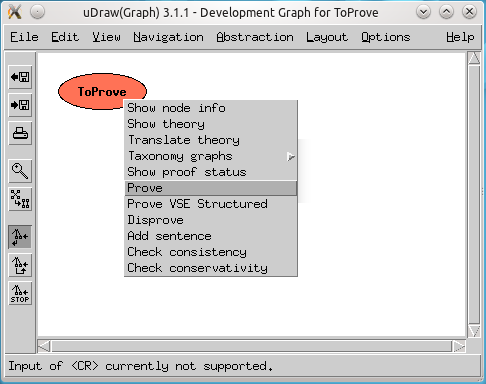
\includegraphics[width=0.5\linewidth,keepaspectratio=true]{UserGuideCL_Prove_devGraph}
  \caption{Prove local proof obligation\label{fig:Prove_devGraph}}
\end{figure}

\begin{figure}[ht]
\begin{minipage}[b]{0.5\linewidth}
  \centering
  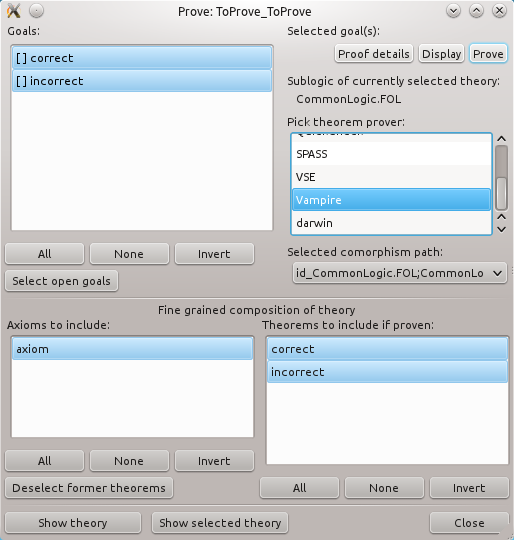
\includegraphics[width=\linewidth,keepaspectratio=true]{UserGuideCL_Prove_Prove}
  \caption{\Hets Goal and Prover Interface\label{fig:proof_window}}
\end{minipage}
\hspace{0.1\linewidth}
\begin{minipage}[b]{0.5\linewidth}
  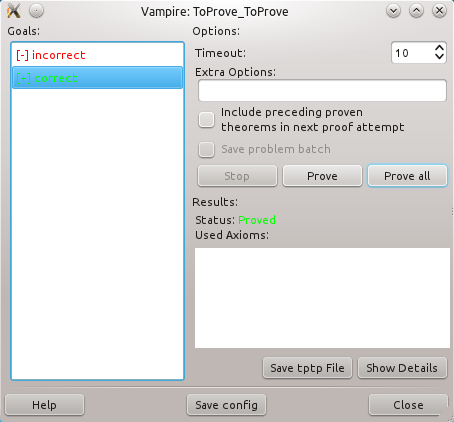
\includegraphics[width=\linewidth,keepaspectratio=true]{UserGuideCL_Prove_Vampire}
  \caption{Interface of Vampire Prover\label{fig:Vampire}}
\end{minipage}
\end{figure}

If you open this GUI when processing the goals of one node for the
first time, it will show all goals as open. Within this list you can
select those goals that should be inspected or proved. The GUI elements are the following:

\begin{itemize}
\item The button `Display' shows the selected goals in the ASCII syntax of
  this theory's logic in a separate window.
\item By pressing the `Proof details' button a window is opened where for each
  proved goal the used axioms, its proof script, and its proof are shown ---
  the level of detail depends on the used theorem prover.
\item With the `Prove' button the actual prover is launched. The provers are described
  in more detail in the \Hets user guide \cite{HetsUserGuide}.
\item The list `Pick Theorem Prover:' lets you choose one of the connected
  provers (among them \Isabelle, MathServe Broker, \SPASS, Vampire, and
  zChaff, described below). By pressing `Prove' the selected prover is
  launched and the theory along with the selected goals is translated via the
  shortest possible path of comorphisms into the prover's logic.
\item The pop-up choice box below `Selected comorphism path:' lets you pick a
  (composed) comorphism to be used for the chosen prover. If the specification
  does not contain any sequence markers, it is possible to use the comorphism
  \texttt{CommonLogic2CASLCompact} which results in a simpler 
  \CASL specification. We recommend using this comorphism whenever possible.
\item Since the amount and kind of sentences sent to an ATP system is a major
  factor for the performance of the ATP system, it is possible to select in
  the bottom lists the axioms and proven theorems that will comprise the
  theory of the next proof attempt. Based on this selection the sublogic may
  vary \ednote{CL: From here, my brain can't parse this sentence.}and also the available provers and comorphisms to provers. Former
  theorems that are imported from other specifications are marked with the
  prefix `(Th)'. Since former theorems do not add additional logical content,
  they may be safely removed from the theory.
\item If you press the bottom-right `Close' button the window is closed and
  the status of the goals' list is integrated into the development graph. If
  all goals have been proved, the selected node turns from red into green.
\item All other buttons control selecting list entries.
\end{itemize}

In order to prove or disprove a theorem, it needs to be declared as proof 
obligation. This is done by the keyword \texttt{\%implied} at the end of a text:

\begin{lstlisting}[morekeywords={logic,spec,and,implied,end}]
logic CommonLogic

spec ToProve =
. (P x)
  (and (P x) (Q y))
. (Q y) %implied %(correct)%
. (P y) %implied %(incorrect)%
end
\end{lstlisting}

In this specification the theorems, annotated (named) by \texttt{correct} and 
\texttt{incorrect} are the ones, that can be proven or disproven.
Note that they are separate texts inside the specification \texttt{ToProve}.
The annotations are optional. For proving, they are the names shown in the 
``Axioms to include'' section of the prover interface 
(Fig.~\ref{fig:proof_window}).

The same specification can be written down in CLIF:
\begin{lstlisting}[language=clif,morekeywords={implied}]
(cl:text axiom
  (P x)
  (and (P x) (Q y))
)

(cl:text correct
  (Q y)
) %implied

(cl:text incorrect (P y)) %implied
\end{lstlisting}
In CLIF, there is no notion of proof obligation. Hence the \texttt{\%implied} 
keyword of \Hets must be used, and thus the specification is not pure CLIF. Because the texts have 
names, these are also used in the prover interface. Otherwise, \Hets invents 
names.

\subsection{Consistency Checker}
\label{sec:CC}
Since proofs are void if specifications are inconsistent, the consistency
should be checked (if possible for the given logic) by the ``Consistency
checker'' shown in Fig.~\ref{fig:cons_window}.  This GUI is invoked from
the `Edit' menu as it operates on all nodes.

The list on the left shows all node names prefixed with a consistency status
in square brackets that is initially empty.  A consistent node is indicated by
a `+', a `–' indicates an inconsistent node, a `t' denotes a timeout of the last
checking attempt.

\begin{figure}[ht]
\begin{minipage}[b]{0.5\linewidth}
  \centering
  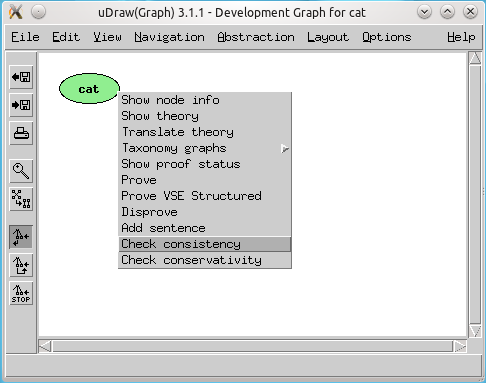
\includegraphics[width=\linewidth,keepaspectratio=true]{UserGuideCL_Consistency_devGraph}
  \caption{Selection of consistency checker\label{fig:cons_devGraph}}
\end{minipage}
\hspace{0.1\linewidth}
\begin{minipage}[b]{0.5\linewidth}
  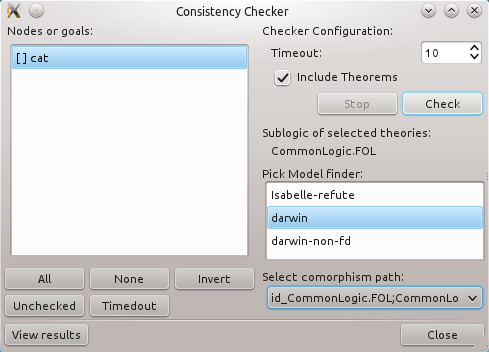
\includegraphics[width=\linewidth,keepaspectratio=true]{UserGuideCL_Consistency_Interface}
  \caption{\Hets Consistency Checker Interface\label{fig:cons_window}}
\end{minipage}
\end{figure}


For some selection of nodes (of a common logic) a model finder should be
selectable from the `Pick Model finder:' list. Currently only for ``darwin''
some \CASL models can be re-constructed. When pressing `Check', possibly after
`Select comorphism path:', all selected nodes will be checked, spending at
most the number of seconds given under `Timeout:' on each node. Pressing
`Stop' allows to terminate this process if too many nodes have been chosen.
Either by `View results' or automatically the `Results of consistency check'
(Fig.~\ref{fig:cons_res}) will pop up and allow you to inspect the models for
nodes, if they could be constructed.

\begin{figure}[ht]
  \centering
  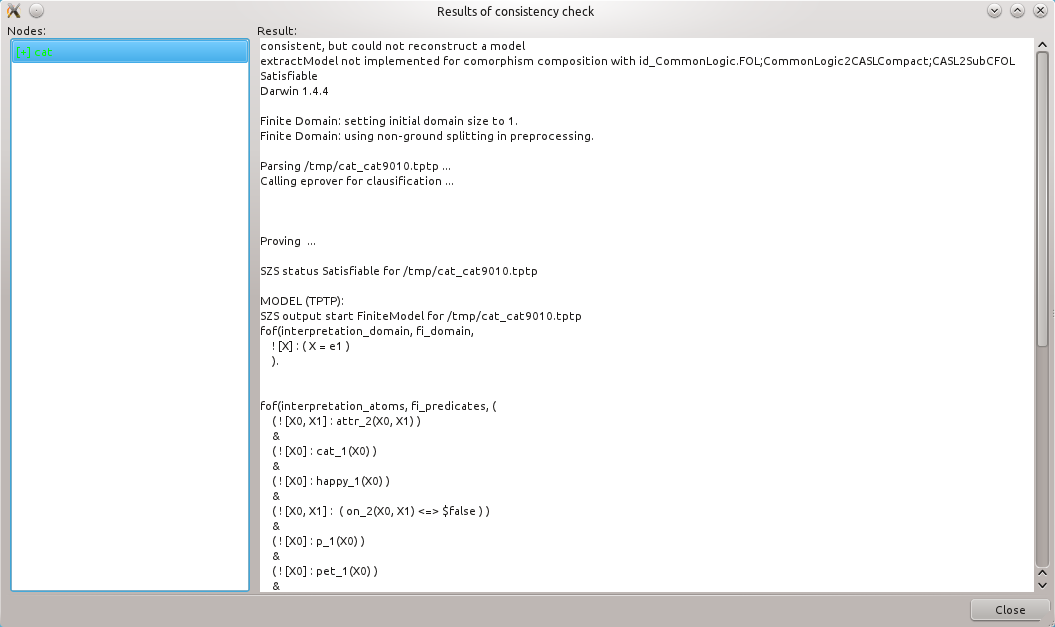
\includegraphics[width=0.75\linewidth,keepaspectratio=true]{UserGuideCL_Consistency_Result}
  \caption{Consistency checker results\label{fig:cons_res}}
\end{figure}

\subsection[Automated Theorem Proving Systems]
{Automated Theorem Proving Systems\\(Logic SoftFOL)}
\label{sec:ATP}

\begin{figure}
\centering
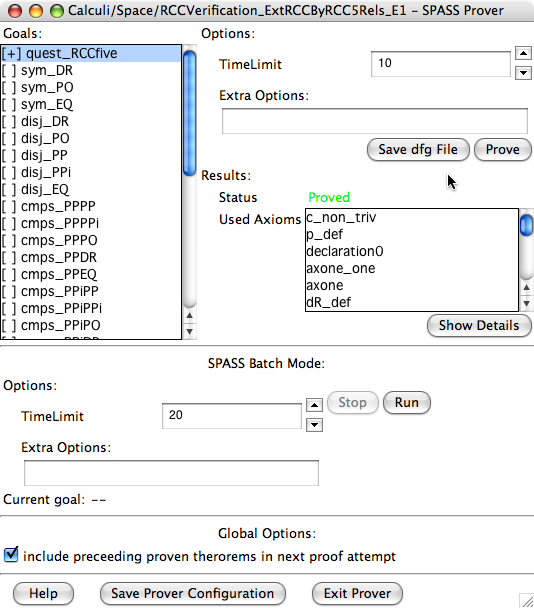
\includegraphics[width=\textwidth]{spassGUI1}
\caption{Interface of the \SPASS prover\label{fig:SPASS_GUI}}
\end{figure}

All ATPs integrated into \Hets share the same GUI, with only a slight
modification for the MathServe Broker: the input field for extra options is
inactive. Fig.~\ref{fig:SPASS_GUI} shows the instantiation for \SPASS, where
in the top right part of the window the batch mode can be controlled.  The
left side shows the list of goals (with status indicators).  If goals are
timed out (indicated by `t') it may help to activate the check box `Include
preceding proven theorems in next proof attempt' and pressing `Prove all'
again.

On the bottom right the result of the last proof
attempt is displayed.  The `Status:' indicates `Open', `Proved', `Disproved',
`Open (Time is up!)', or `Proved (Theory inconsistent!)'. The list of `Used
Axioms:' is filled by \SPASS. The button `Show Details' shows the whole output
of the ATP system. The `Save' buttons allow you to save the input and
configuration of each proof for documentation. By `Close' the results for all
goals are transferred back to the Proof Management GUI.

The MathServe system \cite{ZimmerAutexier06} developed by J\"{u}rgen
Zimmer provides a unified interface to a range of different ATP
systems; the most important systems are listed in
Tab.~\ref{tab:MathServe}, along with their capabilities. These
capabilities are derived from the \emph{Specialist Problem Classes}
(SPCs) defined upon the basis of logical, language and syntactical
properties by Sutcliffe and Suttner \cite{SutcliffeEA:2001:EvalATP}.
Only two of the Web services provided by the MathServe system are used
by \Hets currently: Vampire and the brokering system.  The ATP systems
are offered as Web Services using standardised protocols and formats
such as SOAP, HTTP and XML.  Currently, the ATP system Vampire may be
accessed from \Hets via MathServe; the other systems are only reached
after brokering.

\begin{table}[t]
  \centering
  \begin{threeparttable}
    \begin{tabular}{|l|c|p{7cm}|}\firsthline
      ATP System & Version & Suitable Problem Classes\tnote{a}\\
      \hhline{|=|=|=|}
      DCTP & 10.21p & effectively propositional \\\hline
      EP & 0.91 & effectively propositional; real first-order, no
      equality; real first-order, equality\\\hline
      Otter & 3.3 & real first-order, no equality\\\hline
      \SPASS & 2.2 & effectively propositional; real first-order, no
      equality; real first-order, equality\\\hline
      Vampire & 8.0 & effectively propositional; pure equality, equality
      clauses contain non-unit equality clauses; real first-order, no
      equality, non-Horn\\\hline
      Waldmeister & 704 & pure equality, equality clauses are unit
      equality clauses\\\lasthline
    \end{tabular}
    %\renewcommand{\thempfootnote}{\arabic{mpfootnote}}
    %\footnotetext%[\value{footnote}\stepcounter{footnote}]
    \begin{tablenotes}\footnotesize
    \item[a]
      {The list of problem classes for each ATP system is not
        exhaustive, but only the most appropriate problem classes are
        named according to benchmark tests made with MathServe by
        J\"urgen Zimmer.}
    \end{tablenotes}
  \end{threeparttable}
  \caption{ATP systems provided as Web services by MathServe}
\vspace*{-4mm}
  \label{tab:MathServe}
\end{table}

For details on the ATPs supported, see the \Hets user guide \cite{HetsUserGuide}.

\section{Reading, Writing and Formatting}

\Hets provides several options controlling the types of files
that are read and written.
\begin{description}
\item[\texttt{-i ITYPE}, \texttt{-{}-input-type=ITYPE}] Specify \texttt{ITYPE}
  as explicit type of the input file. 

  \texttt{exp} files contain a development graph in a new experimental OMDoc
  format.  \texttt{prf} files contain additional development steps (as shared
  ATerms) to be applied on top of an underlying development graph created from
  a corresponding \texttt{env}, \texttt{casl}, or \texttt{het}
  file. \texttt{hpf} files are plain text files representing heterogeneous
  proof scripts. The contents of a \texttt{hpf} file must be valid input for
  \Hets in interactive mode.  (\texttt{gen\_trm} formats are currently not
  supported.)

The possible input types are:
\begin{lstlisting}
    casl
  | het
  | owl
  | hs
  | exp
  | maude
  | elf
  | hol
  | prf
  | omdoc
  | hpf
  | clf
  | clif
  | xml
  | [tree.]gen_trm[.baf]
\end{lstlisting}

\item[\texttt{-O DIR}, \texttt{-{}-output-dir=DIR}]
Specify \texttt{DIR} as destination directory for output files.

\item[\texttt{-o OTYPES}, \texttt{-{}-output-types=OTYPES}]
\texttt{OTYPES} is a comma-separated list of output types:
\begin{lstlisting}
    prf
  | env
  | omn
  | clif
  | omdoc
  | xml
  | exp
  | hs
  | thy
  | comptable.xml
  | (sig|th)[.delta]
  | pp.(het|tex|xml|html)
  | graph.(exp.dot|dot)
  | dfg[.c]
  | tptp[.c]
\end{lstlisting}
The \texttt{env} and \texttt{prf} formats are for subsequent reading,
avoiding the need to re-analyse downloaded libraries. \texttt{prf} files
can also be stored or loaded via the GUI's File menu.

The \texttt{omn} option \cite{w3c:owl2-manchester} will produce OWL files in
Manchester Syntax for each specification of a structured OWL library.

The \texttt{clif} option will produce Common Logic files in
CLIF dialect for each specification of a Common Logic library.

The \texttt{omdoc} format \cite{books/sp/Kohlhase06} is an XML-based
markup format and data model for Open Mathematical Documents. It
serves as semantics-oriented representation format and ontology
language for mathematical knowledge. Although this is still in experimental 
state, Common Logic theories can be exported to and imported from OMDoc.

The \texttt{xml} option will produce an XML-version of the development graph
for our change management broker.

The \texttt{exp} format is the new experimental omdoc format.

The \texttt{hs} format is used for Haskell modules. Executable \CASL or
\HasCASL specifications can be translated to Haskell.

When the \texttt{thy} format is selected, \Hets will try to translate
each specification in the library to \Isabelle, and write one \Isabelle
\texttt{.thy} file per specification.

When the \texttt{comptable.xml} format is selected, \Hets will extract
the composition and inverse table of a Tarskian relation algebra from
specification(s) (selected with the \texttt{-n} or \texttt{-{}-spec}
option). It is assumed that the relation algebra is
generated by basic relations, and that the specification is written
in the \CASL logic. A sample specification of a relation
algebra can be found in the \Hets library \texttt{Calculi/Space/RCC8.het},
available from \url{http://www.cofi.info/Libraries}.
The output format is XML, the URL of the DTD is included in the
XML file.

The \texttt{sig} or \texttt{th} option will create \HetCASL signature or
theory files for each development graph node. (The \texttt{.delta} extension
is not yet supported.)

The \texttt{pp} format is for pretty printing, either as plain text
(\texttt{het}), \LaTeX\ input (\texttt{tex}), HTML (\texttt{html}) or XML
(\texttt{xml}).  For example, it is possible to generate a pretty printed
\LaTeX\ version of \texttt{Cat.clif} by typing:

\begin{quote}
\texttt{hets -v2 -o pp.tex Cat.clif}
\end{quote}

This will generate a file \texttt{Cat.pp.tex}. It can be included
into \LaTeX\ documents, provided that the style \texttt{hetcasl.sty}
coming with the \Hets distribution (\texttt{LaTeX/hetcasl.sty}) is used.

The format \texttt{pp.xml} represents just a parsed library in XML.

Formats with \texttt{graph} are reserved for future usage.

The \texttt{dfg} format is used by the \SPASS theorem prover
\cite{WeidenbachEtAl02}.

The \texttt{tptp} format (\url{http://www.tptp.org}) is a standard
exchange format for first-order theorem provers.

Appending \texttt{.c} to \texttt{dfg} or \texttt{tptp} will create files for
consistency checks by SPASS or Darwin respectively.

For all output formats it is recommended to increase the verbosity to at least
level 2 (by using the option \texttt{-v2}) to get feedback which files are
actually written. (\texttt{-v2} also shows which files are read.)

\item[\texttt{-t TRANS}, \texttt{-{}-translation=TRANS}]
chooses a translation option. \texttt{TRANS} is a colon-separated list
without blanks of one or more comorphism names (see Sect.~\ref{comorphisms})

\item[\texttt{-n SPECS}, \texttt{-{}-spec=SPECS}]
chooses a list of named specifications for processing

\item[\texttt{-w NVIEWS}, \texttt{-{}-view=NVIEWS}]
chooses a list of named views for processing

\item[\texttt{-R}, \texttt{-{}-recursive}] output also imported libraries

\item[\texttt{-I}, \texttt{-{}-interactive}] run \Hets in interactive mode

\item[\texttt{-X}, \texttt{-{}-server}] run \Hets as web server (see
  Sect.~\ref{sec:Server})

\item[\texttt{-x}, \texttt{-{}-xml}] use XML-PGIP\footnote{Proof General Interface Protocol} packets to communicate with
  \Hets in interactive mode

\item[\texttt{-S PORT}, \texttt{-{}-listen=PORT}] communicate
  with \Hets in interactive mode by listening to the port \texttt{PORT}

\item[\texttt{-c HOSTNAME:PORT}, \texttt{-{}-connect=HOSTNAME:PORT}] communicate
  with \Hets in interactive mode via connecting to the port on host
  \texttt{HOSTNAME}

\item[\texttt{-d STRING}, \texttt{-{}-dump=STRING}] produces implementation
  dependent output for debugging purposes only
  (i.e.\ \texttt{-d LogicGraph} lists the logics and comorphisms)
\end{description}

\section{Hets as a web server}\label{sec:Server}

Large parts of \Hets are now also available via a web interface. A running
server should be accessible on
\url{http://pollux.informatik.uni-bremen.de:8000/}. It allows to browse the
\Hets library, upload a file or just a \HetCASL specification. Development
graphs for well-formed specifications can be displayed in various formats
where the \texttt{svg} format is supposed to look like the graphs displayed by
uDrawGraph. Besides browsing, the web server is supposed to be accessed by
other programs using queries. The possible queries are described at
\url{http://trac.informatik.uni-bremen.de:8080/hets/wiki/RESTfulInterface}.

For details on this topic, see the \Hets user guide \cite{HetsUserGuide}.

\section{Miscellaneous Options}

\begin{description}
\item[\texttt{-v[Int]}, \texttt{-{}-verbose[=Int]}]
Set the verbosity level according to \texttt{Int}. Default is 1.
\item[\texttt{-q}, \texttt{-{}-quiet}]
Be quiet -- no diagnostic output at all. Overrides -v.
\item[\texttt{-V}, \texttt{-{}-version}] Print version number and exit.
\item[\texttt{-h}, \texttt{-{}-help}, \texttt{-{}-usage}]
Print usage information and exit.
\item[\texttt{+RTS -KIntM -RTS}] Increase the stack size to
 \texttt{Int} megabytes (needed in case of a stack overflow).
This must be the first option.
\item[\texttt{-l LOGIC}, \texttt{-{}-logic=LOGIC}] chooses the initial logic, which is used for processing the specifications before the first \textbf{logic L}
declaration. The default is \CASL.
\item[\texttt{-e ENCODING}, \texttt{-{}-encoding=ENCODING}] Read input files using latin1 or utf8 encoding. The default is still latin1.
\item[\texttt{-{}-unlit}] Read literate input files.
\item[\texttt{-{}-relative-positions}] Just uses the relative library name in positions of warning or errors.
\item[\texttt{-U FILE}, \texttt{-{}-xupdate=FILE}] update a development graph according to special XML update information (still experimental).
\item[\texttt{-m FILE}, \texttt{-{}-modelSparQ=FILE}] model check a qualitative calculus given in SparQ lisp notation \cite{SparQ06} against a \CASL specification
\end{description}


\bibliographystyle{plain}
\bibliography{cofibib,cofi-ann,UM,hets,kl,hetsForCL}
\end{document}

%%% Local Variables:
%%% mode: latex
%%% TeX-master: "UserGuideCommonLogic"
%%% ispell-local-dictionary: "british"
%%% End:
% LocalWords:  SPASS darwin uninger Hets HetCASL SoftFOL EL QL RL zChaff TPTP
% LocalWords:  Eprover KRHyper MathServe CASL THF HasCASL RelScheme CommonLogic
% LocalWords:  CASLCompact CommonLogicModuleElimination SuleCFOL hets oneiric
% LocalWords:  SoftFOLInduction mpkg MacPorts libglade uDraw Tcl Tk bunzip VSE
% LocalWords:  minisat Twelf Attr clif libdir casl het clf Pred PetHappy gui DG
% LocalWords:  uncolored COLORE someFile http https someText someTargetFile sp
% LocalWords:  someTranslationFile someAxiom Nonconservative nonconservative EP
% LocalWords:  libs someOtherFile nextFile andSoOn nameInTargetFile forall iff
% LocalWords:  nameInCurrentFile ToProve ATPs rgen Zimmer SPCs Sutcliffe DCTP
% LocalWords:  Suttner Waldmeister urgen ITYPE OMDoc prf ATerms env hpf trm hs
% LocalWords:  maude hol omdoc xml baf dir OTYPES omn comptable sig th tex html
% LocalWords:  dfg tptp Tarskian hetcasl NVIEWS pgip HOSTNAME LogicGraph svg
% LocalWords:  uDrawGraph RTS KIntM latin utf xupdate modelSparQ SparQ cofibib
% LocalWords:  cofi ann hetsForCL Mossakowski Maeder Mihai Codescu
% LocalWords:  Kuksa DFKI GmbH IEC lang basicstyle morecomment
% LocalWords:  escapeinside importedSpec importingSpec
